\subsection{Database modultest}
Der er som gruppe taget en beslutning om at hoste databasen lokalt i en docker container. Dette blev valgt på baggrund af en samtale med vejleder, hvor vi blandt andet, grundet sikkerhedsforanstaltning på au’s netværk, kunne løbe ind i nogle problemer.
Den lokale hosting medførte at vi kunne holde øje med databasens udformningen, samt den gemte data gennem Microsoft azure datastudie. \newline
For at teste DAL funktioner og dens forbindelse til databasen, oprettes først et DAL objekt med en context som indeholder en korrekt connectionstring.\newline
Til test hvor der skal indsættes data i databasen oprettes der objekter af den korrekte type hvorefter DAL funktioner til indsættes kaldes. Korrektheden af de indsatte data kan herefter tjekkes med datastudie.
\newline
Et eksempel på dette kan ses på figur xx herunder.
Der oprettes et DAL objekt, datahelper, og et GameDTO objekt, gamesave.
Her opsættes gamesave til ”Gamer1”, med navnet ”My First Run”, hvorefter der tilføjes yderligere data. Det overskrevne save er ”NewGame1”, som her har id 1.

\begin{figure}[H]
\centering
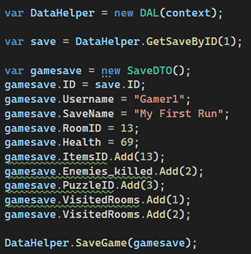
\includegraphics[width = 0.5\textwidth]{02-Body/Images/DAL-Database/NewSave.png}
\caption{Kode til test af SaveGame}
\label{fig:SaveGame-test}
\end{figure}

På figur xxx herunder ses et screenshot fra datastudie hvor de 5 saves til ”Gamer1” kan ses.
Det noteres at alle saves er ”blanke” og starter i rum 1.

\begin{figure}[H]
\centering
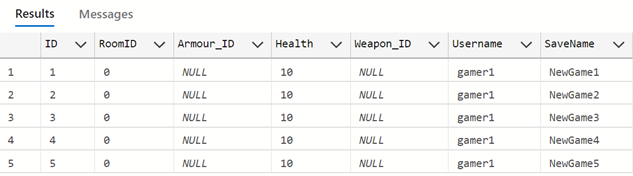
\includegraphics[width = 0.5\textwidth]{02-Body/Images/DAL-Database/DatastudieFørIndsættelse.png}
\caption{}
\label{fig:}
\end{figure}

Herefter køres programmet fra figur xx(kode), og vi kan nu se ændringerne i databasen.
Det noteres at SaveName og de andre attributter nu er opdateret korrekt efter koden.

\begin{figure}[H]
\centering
\includegraphics[width = 0.5\textwidth]{02-Body/Images/DAL-Database/DataStudieEfterIndsættelse.png}
\caption{}
\label{fig:}
\end{figure}

Øvrige lister er også opdateret korrekt, som set på figur xx herunder.

\begin{figure}[H]
\centering
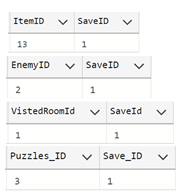
\includegraphics[width = 0.3\textwidth]{02-Body/Images/DAL-Database/Lister.png}
\caption{}
\label{fig:}
\end{figure}

Funktioner hvor der skal læses fra Db kaldes DAL funktionen hvorefter den fundne information udskrives til konsolen ved hjælp af console writeline. Korrektheden af data i konsolen dobbelttjekkes med datastudie.
Et eksempel på dette ses på figur xx herunder.
Her henter vi de gemte save fra tidligere fra ”Gamer1” ved navn ”My First Run”, hvorefter data fra dette save udskrives i konsolen.


\begin{figure}[H]
\centering
\includegraphics[width = 0.5\textwidth]{02-Body/Images/DAL-Database/KodeTilLæsning.png}
\caption{}
\label{fig:KodeTilLæsningAfSave}
\end{figure}

Når kodestykket ovenfor køres får vi resultatet i konsol som set på figur xx herunder.
Det noteres at det udskrevne data stemmeroverens med det indsatte data fra den tidligere funktionstest.

\begin{figure}[H]
\centering
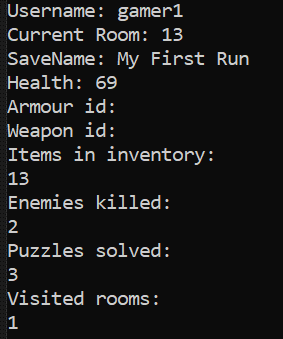
\includegraphics[width = 0.5\textwidth]{02-Body/Images/DAL-Database/ConsoleOutput.png}
\caption{Konsoleudskrift efter læsning af spil fra databasen}
\label{fig:Modulttest-consoleOutput}
\end{figure}


\begin{table}[H]
\begin{tabular}{|p{0.75cm}|p{3.75cm}|p{3.5cm}|p{3.5cm}|p{1.75cm}|} \hline
 \textbf{Test} & \textbf{Funktion} & \textbf{Forventet resultat} & \textbf{Observering} & \textbf{Vurdering} \newline \textbf{(OK/Fail)}\\\hline
 1 & GetRoomDescription(id) & Her forventes det at funktionen henter beskrivelsen fra den valgte rumId. & Funktionen henterbeskrivelsen korrekt og vi kan udskrive denne på konsolen. & OK \\ \hline
 2 & GetAllSaves & Det forventes at alle spillets saves, med tilhørende info, hentes fra databasen & Alle saves hentes fra databasen og information om disse kan udskrives på konsolen. & OK \\ \hline
 3 & GetSaveById(id) & Det forventes at der hentes alle oplysninger om et enkelt save fra databasen med tilsvarende id, som den medsendte parameter & Det korrekte save samt tilhørende info hentes og kan udskrive til konsolen & OK \\ \hline
 4 & SaveGame(Game) & Det forventes at det valgte save med samme id som det nye, overskrives, og at tilhørende info opdateres & Det observeres at det gamle save med samme id, nu er ændret og har korrekte nye værdier & OK \\ \hline
\end{tabular}
\end{table}

